%% =====================================================================
%%  III.  The MA-ZeroPhish framework
%%
%%  One file per main section.  The last subsection of this section is not
%%  here: it is limitations in the full build and capture conduct in the
%%  design build, so the roots input it, which is where an ordering
%%  decision belongs.
%% =====================================================================

% ---- system-overview ---------------------------------------------------

\section{The MA-ZeroPhish Framework}
\label{sec:design}

\subsection{System Model}
\label{sec:overview}

MA-ZeroPhish is an adaptive agentic multi-agent
framework for zero-day phishing detection. Given
a URL or SMS/email message, it produces a verdict
in $\{\mathsf{phishing},\mathsf{benign},
\mathsf{insufficient}\}$ and an evidence-supported
explanation. As illustrated in
Fig.~\ref{fig:pipeline}, the framework consists
of the following core entities.


\begin{figure*}[!t]
    \centering
    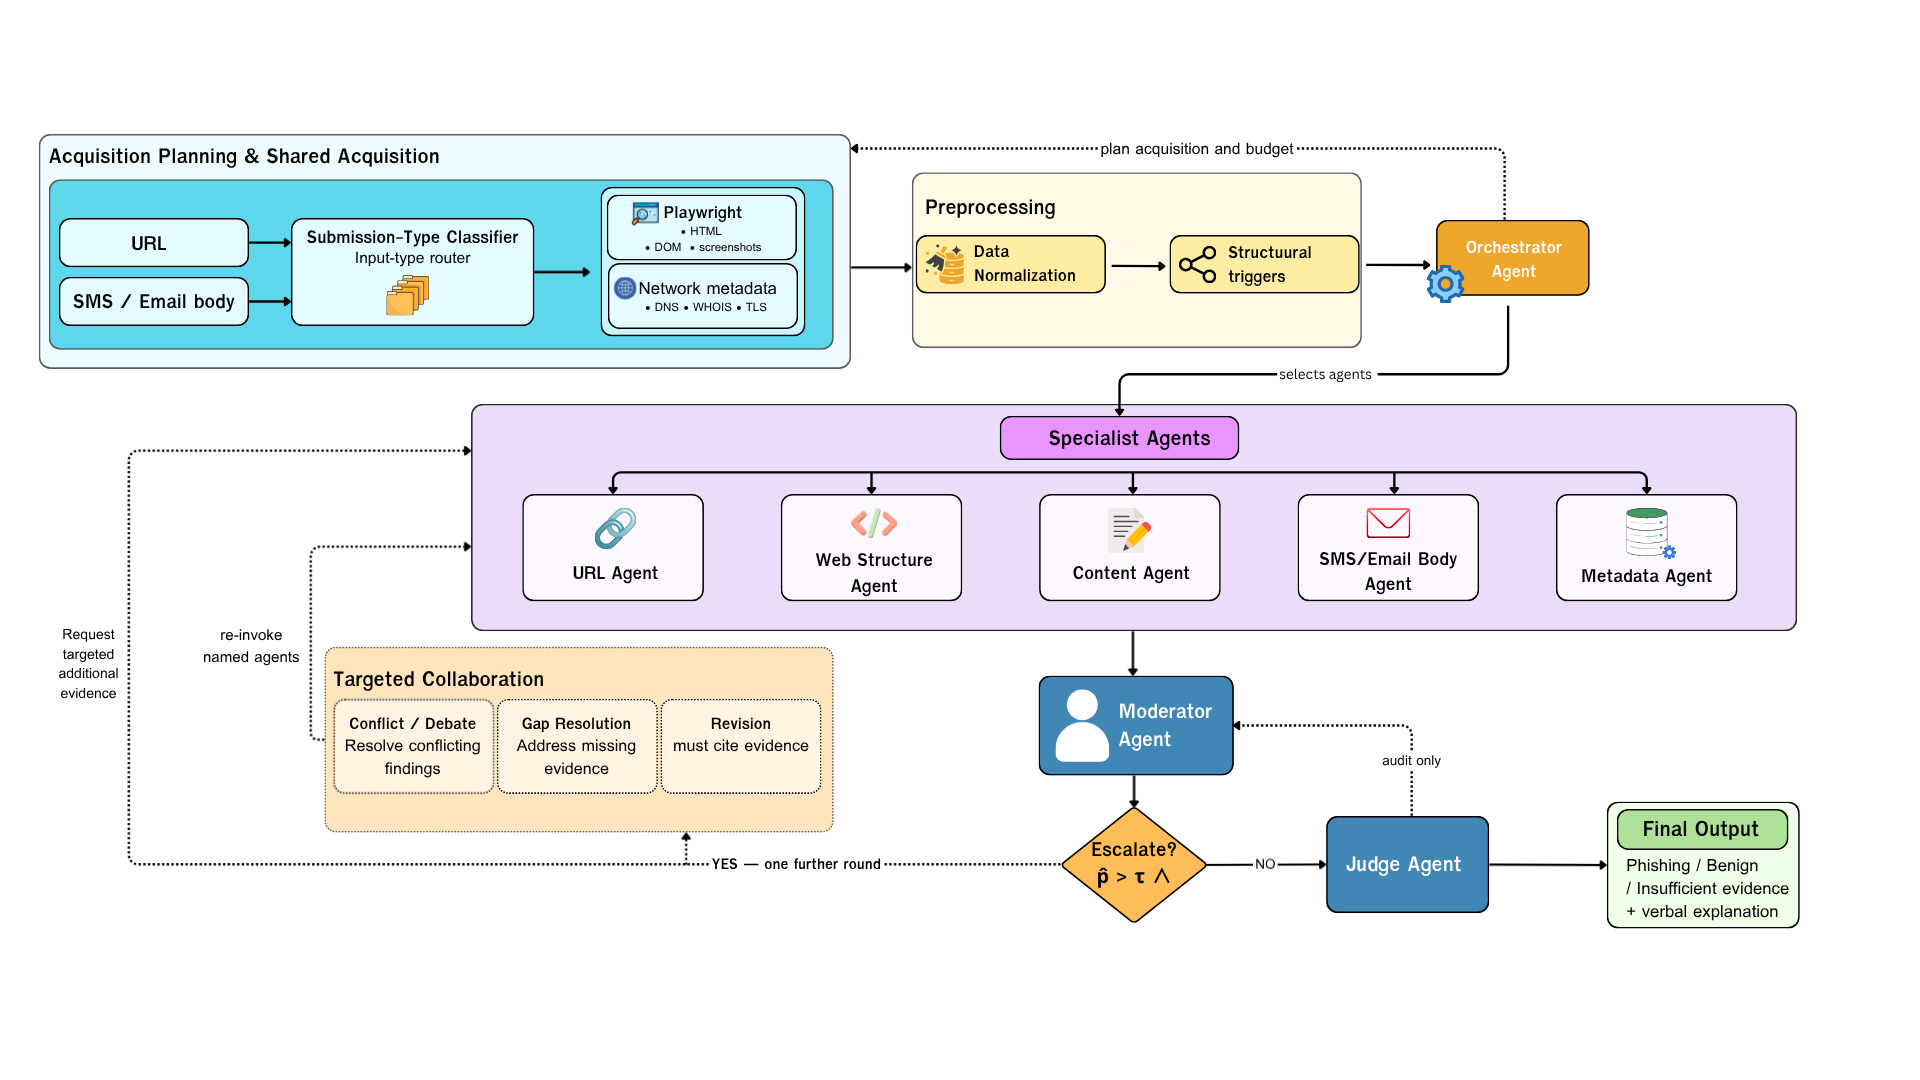
\includegraphics[width=\textwidth]{sections/figures/MA-ZP.png}
    \caption{System architecture of MA-ZeroPhish.}
    \label{fig:pipeline}
\end{figure*}


\begin{itemize}

\item \textbf{Input Classifier (IC):}
Identifies the submission type and determines
the applicable evidence sources without
assessing maliciousness.

\item \textbf{Orchestrator (OR):}
Coordinates budgeted shared evidence acquisition,
normalizes acquired artifacts, and dynamically
selects applicable specialists. It assigns
additive investigation focuses based on
structural evidence conditions but cannot
classify submissions or access specialist
findings.

\item \textbf{Modality-Specialized Agents (MSAs):}
Five agents independently examine complementary
modalities: the URL Agent analyzes lexical
and structural URL properties; the Web Structure
Agent compares served HTML and rendered DOM;
the Content Agent examines rendered text and
visual presentation; the SMS/Email Agent
analyzes message content and requested actions;
and the Metadata Agent investigates DNS,
registration, TLS, and hosting information.
Each agent has a declared tool set and produces
structured findings containing individually
traceable evidence items.

\item \textbf{Moderator (MD):}
Coordinates evidence-driven collaboration
after initial specialist analysis. It reconciles
findings, discounts common-cause evidence,
identifies unresolved conflicts and coverage
gaps, and estimates decision error. Additional
reasoning is initiated only when the estimated
error exceeds a calibrated threshold and an
actionable evidence issue remains. The Moderator
selectively re-invokes relevant agents but
cannot issue the final verdict.

\item \textbf{Judge (JG):}
Independently adjudicates validated item-level
evidence and the coverage report without
accessing specialist verdicts or confidence
bands. It produces the final verdict, supporting
evidence, and explanation but cannot initiate
further investigation.

\end{itemize}


\subsection{Threat Model}
\label{sec:threat}

MA-ZeroPhish considers an adversary
$\mathcal A$ who constructs previously unseen
phishing URLs, webpages, or SMS/email messages
to induce credential disclosure or other
unauthorized user actions while evading
detection. The adversary may control the
submitted content and attacker-operated
infrastructure but cannot directly modify
the framework's acquisition records,
agent configurations, or control logic.
We consider the following capabilities.

\begin{itemize}

\item \textbf{A1: Coordinated Cross-Modal
Manipulation.}
$\mathcal A$ may coordinate URL strings,
webpage structure, rendered content, and
message text to present mutually consistent
but deceptive information. Such observations
may originate from a single attacker-controlled
choice rather than independent evidence,
potentially inflating inter-agent agreement.

\item \textbf{A2: Abuse of Legitimate
Infrastructure.}
$\mathcal A$ may host phishing content on
legitimate cloud services, compromised
websites, or trusted hosting platforms.
Consequently, valid TLS certificates,
established domain registration, and
reputable hosting infrastructure do not
necessarily establish the legitimacy of
the submitted content.

\item \textbf{A3: Template Reuse and
Content Variation.}
$\mathcal A$ may reuse phishing kits across
different campaigns or modify their visual
presentation, URL structure, and message
content. These variations can reduce the
reliability of previously learned features
and create inconsistent evidence across
specialized agents.

\item \textbf{A4: Acquisition Evasion
and Cloaking.}
$\mathcal A$ may block automated browsers,
introduce challenges, or conditionally
serve content according to the requesting
client. Explicit acquisition failures
are recorded as coverage gaps rather than
interpreted as benign evidence. However,
undetected substitution of benign content
for the phishing page may still mislead
the framework.

\item \textbf{A5: Prompt Injection
and Reasoning Manipulation.}
$\mathcal A$ may embed adversarial
instructions in webpage or message content
to influence language-model agents,
suppress suspicious findings, or induce
unsupported inter-agent agreement.
MA-ZeroPhish restricts cross-agent
communication to structured evidence
records and validates evidence references
during revisions. These controls limit
unsupported protocol-level manipulation
but cannot guarantee that an agent
correctly interprets every adversarial
artifact.

\end{itemize}

\noindent\textbf{Security Objectives.}
Under these capabilities, MA-ZeroPhish
aims to maintain traceable evidence
provenance, prevent common-cause
observations from being counted as
independent corroboration, distinguish
acquisition failures from benign findings,
and require evidence-supported inter-agent
revisions. Adaptive collaboration is
intended to resolve actionable conflicts
and evidence gaps without relying solely
on agent consensus or self-reported
confidence.

\noindent\textbf{Scope and Limitations.}
The framework targets previously unseen
phishing attacks that are absent from
system configuration data and available
reputation sources at evaluation time,
and are first observed after the underlying
models' stated knowledge cutoffs.
The cutoff condition does not establish
complete absence from model pretraining.
Attacks against model providers, compromise
of internal framework components, and
network-level attacks on the detector
itself are outside the present scope.
Furthermore, evidence-linked validation
does not eliminate plausible but incorrect
agent interpretations or reliably detect
all forms of content substitution.



\subsection{Modality-Specialized Agents}
\label{sec:specialists}

MA-ZeroPhish employs five modality-specialized
agents with distinct analytical responsibilities,
declared acquisition capabilities, and a common
evidence-reporting contract. Each agent combines
a language-model reasoning component with
modality-specific analytical tools and, where
applicable, an internal machine-learning model.

\begin{definition}[Modality-Specialized Agent]
A specialist agent $g\in\mathcal G$ is defined as
\begin{equation}
g=(\mathcal M_g,\mathcal F_g,\mathcal U_g,
\Psi_g,\mathcal R_g),
\label{eq:agent-definition}
\end{equation}
where $\mathcal M_g$ denotes its analytical
modality, $\mathcal F_g$ its authorized
evidence fields, $\mathcal U_g$ its declared
acquisition tools, $\Psi_g$ its structural
tool-execution predicates, and $\mathcal R_g$
its evidence-based reasoning procedure.
Each agent independently produces a
structured finding record under the common
validation contract of Phase 2.
\end{definition}

The five specialists and their respective
analytical and acquisition capabilities
are summarized in Table~\ref{tab:specialists}.

\begin{table}[!t]
\caption{Specialist Agents and Declared Capabilities}
\label{tab:specialists}
\centering
\scriptsize
\renewcommand{\arraystretch}{1.12}
\setlength{\tabcolsep}{3pt}
\begin{tabular}{p{0.20\columnwidth}
                p{0.35\columnwidth}
                p{0.35\columnwidth}}
\toprule
\textbf{Agent} &
\textbf{Analytical Responsibility} &
\textbf{Additional Acquisition} \\
\midrule
URL &
Pre-render lexical and structural
URL analysis &
Redirect chain \\
\addlinespace
Web Structure &
Served HTML versus rendered
DOM divergence &
Named page-referenced resources \\
\addlinespace
Content &
Rendered presentation versus
markup declaration &
Runtime brand-reference material \\
\addlinespace
SMS/Email &
Message intent and requested
recipient actions &
Supplementary processing of
message-extracted links \\
\addlinespace
Metadata &
DNS, registration, TLS, and
hosting-record structure &
Fresh DNS, registration, TLS,
CT, and hosting records \\
\bottomrule
\end{tabular}
\end{table}

\noindent\textbf{Agent Operating Constraints.}
All specialists follow three common
constraints. First, initial reasoning
is independent, with no access to peer
findings or confidence bands. Second,
supplementary acquisition is restricted
to declared tools and structurally
authorized conditions. Third, every
reported observation must reference
an authorized artifact and an
artifact-specific locator.

The URL Agent does not use blacklist
membership as a detection feature.
The Web Structure Agent focuses on
structural divergence rather than
supervised phishing-label prediction.
The Content Agent preserves text-image
disagreements as separate observations.
The SMS/Email Agent examines the submitted
message without relying on unavailable
conversation history. The Metadata Agent
does not treat certificate issuer,
certificate validity duration, or
legitimate platform infrastructure as
standalone indicators of phishing
or benignity.

The agents may examine overlapping
evidence, but such observations are
not presumed independent. Phase 3
reconciles their causal dependencies
before collaborative reasoning, while
Phase 4 independently adjudicates
their validated observations.


\subsection{System Process}
\label{sec:process}

MA-ZeroPhish operates through four phases:
adaptive evidence acquisition, independent
specialist analysis, evidence-governed
collaboration, and independent adjudication.
The phases separate evidence collection,
agent reasoning, collaboration control,
and final decision-making while preserving
traceable evidence across the workflow.



\subsubsection*{\textbf{Phase 1: Adaptive Shared
Evidence Acquisition and Preparation}}
\label{sec:phase1}

Phase 1 constructs a provenance-tracked
evidence base and determines the initial
specialist configuration. The Orchestrator
coordinates shared acquisition and selects
specialists using structural evidence
conditions without performing phishing
classification.

\medskip
\noindent\textbf{Step 1: Submission Classification
and Acquisition Planning.}
Given a submission $x$, the Input Classifier
assigns a case identifier $cid_x$ and determines
its type
$t_x\in\{\mathsf{URL},\mathsf{SMS},\mathsf{Email}\}$.
A URL submission defines one assessed object.
For SMS/email submissions, the original message
defines a parent object $o_0$, while embedded
URLs are extracted in reading order and assigned
distinct object identifiers $o_i$. All objects
retain $cid_x$ and their parent--child
relationships. Message-level evidence is
preserved even when no URL is extracted.

For each object $o_i$, let $\mathcal S_i$
denote its applicable evidence sources and
$\mathcal I_i$ the required acquisition
instruments. The Orchestrator constructs
\begin{equation}
\mathcal P_i=
(\mathcal S_i,\mathcal I_i,B_i,r_{\max}),
\label{eq:acquisition-plan}
\end{equation}
where $B_i$ is the object's allocated shared
acquisition budget and $r_{\max}$ is the
maximum number of attempts per instrument,
including the initial attempt.

A case-wide budget $B_x$ is partitioned
among shared acquisition, initial specialist
execution, and subsequent collaboration:
\begin{equation}
\begin{aligned}
B_x={}&B_x^{\mathrm{shared}}
+B_x^{\mathrm{agent}}
+B_x^{\mathrm{coll}},\\
&\sum_i B_i\leq B_x^{\mathrm{shared}}.
\end{aligned}
\label{eq:case-budget}
\end{equation}
The Orchestrator maintains a case-wide ledger
of committed and consumed costs. Shared
artifacts are acquired once when reusable
across objects, and their costs are charged
only once. Budget transfers, if permitted,
must be recorded before further commitments.

Browser and URL-dependent network acquisition
require an available URL, whereas original
message evidence can be processed independently.

\medskip
\noindent\textbf{Step 2: Instrument-Level
Evidence Acquisition.}
For each instrument $j\in\mathcal I_i$,
the Orchestrator maintains
\begin{equation}
A_{i,j}=
(st_{i,j},n_{i,j},c_{i,j}),
\label{eq:acquisition-state}
\end{equation}
where $st_{i,j}$ denotes its execution state,
$n_{i,j}$ its attempt count, and $c_{i,j}$
its accumulated cost.

An attempt $a$ using instrument $j$ is
permitted only when
\begin{equation}
\begin{aligned}
\mathsf{Permit}(a)={}&
\mathsf{DepsReady}(a)
\land(n_{i,j}<r_{\max})\\
&\land\mathsf{Retryable}(a)
\land\mathsf{BudgetReady}(a),
\end{aligned}
\label{eq:acquisition-permit}
\end{equation}
where $\mathsf{BudgetReady}(a)$ requires
the estimated cost $c(a)$ to fit both
the object's uncommitted allocation and
the case-wide shared-acquisition balance.
The cost is reserved atomically before
execution and reconciled against measured
expenditure afterward.

The retry predicate permits initial
attempts, retries following transient
failures, and predefined alternative
procedures. Every attempted procedure
counts toward the corresponding instrument
limit and consumes its measured cost,
including unsuccessful attempts.

A shared browser acquisition may produce
served HTML, rendered DOM, webpage content,
and screenshots, and is performed by a
scripted headless browser. Separate
instruments retrieve network metadata when
applicable, returning DNS, registration,
TLS, Certificate Transparency, and hosting
records. Each instrument is specified by
the record set it must return rather than
by its implementation, so substituting a
tool that returns the same records is a
configuration change and not a design
change.
Instrument outcomes and source availability
are recorded independently, permitting
partial success without treating every
missing artifact as a separate failure.

Acquisition terminates when all applicable
sources are obtained, no further attempt
is authorized, or the allocated budget
is exhausted.

\medskip
\noindent\textbf{Step 3: Evidence Normalization
and Provenance Binding.}
Acquired artifacts are normalized into
the evidence envelope
\begin{equation}
E_i=
(o_i,cid_x,\mathcal D_i,\mathcal V_i,
\mathcal A_i,\mathcal P_i^{\mathrm{prov}}),
\label{eq:evidence-envelope}
\end{equation}
where $\mathcal D_i$ contains normalized
evidence, $\mathcal V_i$ records source
availability, $\mathcal A_i$ contains
instrument outcomes, and
$\mathcal P_i^{\mathrm{prov}}$ stores
artifact provenance.

Each artifact is bound to its source,
instrument, capture identifier, assessed
object, and case identifier. Reused
artifacts retain their original acquisition
identity rather than being represented
as independent captures. Source availability
distinguishes obtained, applicable-but-
unavailable, and inapplicable evidence.
Failed attempts retain their outcomes
and failure reasons.

Artifacts from different captures remain
distinguishable and are not implicitly
treated as simultaneous observations.
Parent-message relationships and shared
artifact identifiers are preserved for
case-wide dependency analysis in Phase 3.

\medskip
\noindent\textbf{Step 4: Structural Triggering
and Adaptive Specialist Selection.}
Let $\mathcal G=\{g_1,\ldots,g_5\}$
denote the specialists defined in
Section~\ref{sec:specialists}. Each agent
$g$ has declared evidence fields
$\mathcal F_g$, tools $\mathcal U_g$,
and structural acquisition predicates
$\Psi_g$.

The Orchestrator constructs
\begin{equation}
\mathcal T_i=
\{\theta=(t,f,f'):
\psi_t(f,f',E_i)=1\},
\label{eq:structural-triggers}
\end{equation}
where $\psi_t$ is a deterministic
predicate over normalized fields.
Supported predicates identify shared
entity tokens, mismatched registrable
hosts, cross-origin references, and
corresponding populated-versus-empty
fields. Each trigger retains its
originating field identifiers and
associated artifact references.

For each specialist, define
\begin{equation}
\mathcal T_{i,g}=
\{\theta\in\mathcal T_i:
\mathsf{Fields}(\theta)
\cap\mathcal F_g\neq\varnothing\}.
\label{eq:agent-trigger-coverage}
\end{equation}

Let $a_{i,g}\in\{0,1\}$ indicate
specialist applicability and
$q_{i,g}\in\{0,1\}$ its readiness:
\begin{equation}
\begin{aligned}
a_{i,g}={}&
\mathsf{Fields}(\mathcal S_i)
\cap\mathcal F_g\neq\varnothing,\\
q_{i,g}={}&
\mathsf{HasEvidence}(g,E_i)\\
&\lor\mathsf{FeasibleAcquire}
(g,E_i,B_{i,g}^{\mathrm{tool}}).
\end{aligned}
\label{eq:agent-readiness}
\end{equation}
Here $B_{i,g}^{\mathrm{tool}}$ is
the proposed local acquisition
reservation. Feasibility requires
a declared tool, a satisfied
structural precondition, and
sufficient uncommitted budget.
Here $\mathsf{Fields}(\mathcal S_i)$
denotes the evidence fields supplied by the
applicable sources of Step 1, so
applicability follows from the submission
type structurally and is recorded with the
fields that established it. Applicability
and readiness are determined without
preliminary phishing judgments.

An inapplicable agent is excluded from
applicable-modality coverage, so a
misassigned $a_{i,g}$ would remove a
modality from the denominator of
$\mathsf{Cov}_i$ rather than lower it.
A $\mathsf{skipped}$ record whose declared
fields are later populated is therefore
raised as a coverage issue in
$\mathcal J_i^{\mathrm{cover}}$, which
keeps the assignment revisable rather than
final.

To prevent redundant dispatch,
the Orchestrator maximizes
structural trigger coverage while
penalizing execution cost:
\begin{equation}
\begin{aligned}
\max_{\{z_{i,g},u_\theta\}}\quad&
\sum_{\theta\in\mathcal T_i}
w_\theta u_\theta
-\mu\sum_{g\in\mathcal G}
c_{i,g}z_{i,g}\\
\mathrm{s.t.}\quad&
u_\theta\leq
\sum_{g:\theta\in\mathcal T_{i,g}}
z_{i,g},\\
&z_{i,g}\leq a_{i,g},\\
&z_{i,g}\leq q_{i,g},\\
&\sum_{g\in\mathcal G}
c_{i,g}z_{i,g}
\leq B_i^{\mathrm{agent}},\\
&\sum_{g\in\mathcal G}
z_{i,g}\geq m_i,\\
&z_{i,g},u_\theta\in\{0,1\}.
\end{aligned}
\label{eq:specialist-selection}
\end{equation}
Here $w_\theta>0$ weights trigger
coverage, $c_{i,g}>0$ includes
estimated execution and reserved
local acquisition costs, and
$\mu>0$ controls the cost penalty.
The initial specialist allocation
$B_i^{\mathrm{agent}}$ is drawn
from the case-wide agent budget.

The minimum dispatch requirement is
\begin{equation}
m_i=
\begin{cases}
1, &
\displaystyle\sum_{g\in\mathcal G}
a_{i,g}q_{i,g}>0,\\
0, & \text{otherwise}.
\end{cases}
\label{eq:minimum-dispatch}
\end{equation}
It ensures at least one applicable,
ready specialist is selected when
a feasible investigation exists.
If the minimum cannot be funded,
the object is marked as having
insufficient investigation resources
rather than violating the budget.
All weights, costs, and minimum
dispatch rules are fixed using
development data.

The selected agents and their
additive investigation focuses are
\begin{equation}
\begin{aligned}
\mathcal G_i
&=\{g\in\mathcal G:z_{i,g}=1\},\\
\mathcal Q_{i,g}
&=\bigcup_{\theta\in\mathcal T_{i,g}}
\left(
\mathsf{Fields}(\theta)
\cap\mathcal F_g
\right).
\end{aligned}
\label{eq:dispatch-focus}
\end{equation}
Each focus contains predefined field
identifiers and guides attention
without restricting the specialist's
full modality analysis or prescribing
a verdict. An empty focus permits
ordinary independent analysis.

Execution and local acquisition costs
are reserved atomically before dispatch.
Unselected applicable agents receive
system-generated
$\mathsf{not\_dispatched}$ records,
allowing the Moderator to reconsider
their selection in Phase 3.
Inapplicable agents receive
$\mathsf{skipped}$ records.

Phase 1 outputs
$(E_i,\mathcal G_i,
\{\mathcal Q_{i,g}\}_{g\in\mathcal G_i})$
together with the updated case-wide
budget ledger for independent
specialist analysis in Phase 2.



\subsubsection*{\textbf{Phase 2: Provenance-Bound
Independent Specialist Reasoning}}
\label{sec:phase2}

Phase 2 executes the specialists selected
in Phase 1. Each agent independently
analyzes its modality under controlled
tool access and produces provenance-bound
findings. A common validator enforces
execution accountability and derives
deterministic evidence-based confidence
bands.

\medskip
\noindent\textbf{Step 1: Specialist Task
Initialization.}
For each $g\in\mathcal G_i$, the
Orchestrator constructs
\begin{equation}
\begin{aligned}
\mathcal E_{i,g}=\big(
&o_i,g,\mathcal D_{i,g},
\mathcal V_{i,g},\\
&\mathcal P_{i,g}^{\mathrm{prov}},
\mathcal Q_{i,g},
B_{i,g}^{\mathrm{tool}}
\big),
\end{aligned}
\label{eq:specialist-envelope}
\end{equation}
where the fields specify the agent's
authorized evidence, source availability,
artifact provenance, additive investigation
focus, and Phase-1-reserved local
acquisition budget. Shared structural
fields are included when required.
The focus does not restrict the agent's
full modality analysis. Peer findings,
verdicts, and confidence bands remain
inaccessible during initial execution.

\medskip
\noindent\textbf{Step 2: Controlled Local
Evidence Acquisition.}
Each specialist uses only its declared
tools $\mathcal U_g$ under structural
predicates $\Psi_g$. An action $u$
is authorized when
\begin{equation}
\begin{aligned}
\mathsf{Allow}_{i,g}(u)={}&
\mathsf{Own}(u,\mathcal U_g)
\land\mathsf{Precond}(u,\mathcal E_{i,g})\\
&\land\mathsf{FreshNeed}(u,E_i)
\land\mathsf{BudgetReady}_{i,g}(u).
\end{aligned}
\label{eq:local-tool-authorization}
\end{equation}
Here, $\mathsf{FreshNeed}$ requires
missing, supplementary, or explicitly
fresh evidence, considering acquisition
targets and capture identifiers.
$\mathsf{BudgetReady}_{i,g}$ requires
the estimated cost to fit the agent's
remaining Phase-1 reservation.

Each authorized attempt records its
trigger, target, outcome, measured
cost, and provenance. The case-wide
ledger reconciles actual expenditure
and releases unused reservations.
Successful artifacts are registered
after acquisition authorization is
verified and before finding validation.
Different captures retain distinct
provenance.

\medskip
\noindent\textbf{Step 3: Independent
Evidence Extraction.}
Each specialist produces
$\mathcal H_{i,g}
=\{h_{i,g}^{1},\ldots,h_{i,g}^{m_g}\}$,
where
\begin{equation}
h_{i,g}^{j}=
(\omega_j,\ell_j,\rho_j,d_j,s_j,p_j).
\label{eq:evidence-item}
\end{equation}
Here, $\omega_j$ is an observation,
$\ell_j$ a declared field,
$\rho_j$ an artifact-specific locator,
$d_j\in\{\mathsf{phishing},
\mathsf{benign},\mathsf{neutral}\}$
its assessed direction,
$s_j\in\{\mathsf{distinctive},
\mathsf{consistent},\mathsf{marginal}\}$
its assessed strength, and $p_j$
its artifact, instrument, and capture
provenance.

Agents distinguish observed absence
from unavailable evidence and derive
preliminary verdicts solely from their
own findings. Direction and strength
are agent assessments, not verified
facts or calibrated probabilities.
Independent execution does not imply
independence of shared artifacts.

\medskip
\noindent\textbf{Step 4: Provenance-Bound
Record Validation.}
Each executed specialist submits
\begin{equation}
\begin{aligned}
R_{i,g}=\big(
&o_i,g,\eta_{i,g},v_{i,g},
\mathcal H_{i,g},\\
&\mathcal B_{i,g},
\mathcal U_{i,g}^{\mathrm{log}},
n_{i,g}^{\mathrm{omit}}
\big),
\end{aligned}
\label{eq:finding-record}
\end{equation}
where $\eta_{i,g}$ is the runtime-assigned
status, $v_{i,g}$ the preliminary
verdict, $\mathcal B_{i,g}$ the
examined fields,
$\mathcal U_{i,g}^{\mathrm{log}}$
the acquisition log, and
$n_{i,g}^{\mathrm{omit}}$ the
number of findings omitted under
the configured reporting limit.

The deterministic validator checks
\begin{equation}
\begin{aligned}
\mathsf{Valid}(R_{i,g})={}&
\mathsf{SchemaValid}(R_{i,g})
\land\mathsf{ScopeValid}(\mathcal H_{i,g})\\
&\land\mathsf{BasisValid}(\mathcal B_{i,g})
\land\mathsf{ToolValid}
(\mathcal U_{i,g}^{\mathrm{log}})\\
&\land\!\!
\bigwedge_{h_j\in\mathcal H_{i,g}}
\mathsf{Resolve}(\ell_j,\rho_j,p_j).
\end{aligned}
\label{eq:record-validity}
\end{equation}
$\mathsf{BasisValid}$ verifies
examined fields against recorded
evidence accesses;
$\mathsf{ToolValid}$ checks tool
authorization and budget compliance;
and $\mathsf{Resolve}$ verifies each
finding's field, locator, and
provenance against the authorized
artifact registry. These checks
establish traceability, not semantic
correctness.

Invalid findings do not enter
subsequent reasoning; rejected
records retain an auditable
$\mathsf{error}$ status.
The runtime distinguishes
$\mathsf{ran}$, $\mathsf{no\_data}$,
$\mathsf{not\_dispatched}$,
$\mathsf{error}$, and $\mathsf{skipped}$.
A completed analysis without
directional evidence remains
$\mathsf{ran}$; $\mathsf{no\_data}$
indicates unavailable required
evidence after permitted acquisition.
Unselected and inapplicable agents
receive system-generated records;
the latter are excluded from
applicable-modality coverage.

\medskip
\noindent\textbf{Step 5: Deterministic
Evidence-Based Confidence.}
For a valid record with directional
verdict $v_{i,g}$, define
\begin{equation}
\begin{aligned}
b_{i,g}=f_{\mathrm{band}}\big(
&\mathsf{Breadth}(\mathcal H_{i,g},v_{i,g}),\\
&\mathsf{Opposition}(\mathcal H_{i,g},v_{i,g}),\\
&\mathsf{TopStrength}(\mathcal H_{i,g},v_{i,g})
\big).
\end{aligned}
\label{eq:record-confidence}
\end{equation}
Breadth counts distinct supporting fields; opposition counts distinct
contrary fields whose assessed strength is at least the top supporting
strength; and top strength is the highest assessed strength among
supporting findings. The fixed mapping assigns $\mathsf{decisive}$ when
top strength is distinctive, breadth is at least two, and opposition is
zero; $\mathsf{strong}$ when top strength is distinctive and opposition is
zero, or top strength is consistent, breadth is at least two, and
opposition is zero; $\mathsf{suggestive}$ when top strength is consistent
and opposition is zero; $\mathsf{thin}$ when at least one supporting field
remains; and $\mathsf{none}$ otherwise. Rules are evaluated in this order,
so the mapping is total.

An inconclusive verdict or invalid
record receives $\mathsf{none}$.
Initial bands exclude borrowed
peer evidence. They summarize
reported support rather than
calibrated correctness probabilities;
agent-specific calibration is applied
to the Moderator's features in
Phase 3. Bands are hidden from
peer specialists and the Judge.

Phase 2 outputs
\begin{equation}
\mathcal R_i=
\{R_{i,g}:g\in\mathcal G\},
\label{eq:phase2-output}
\end{equation}
including system-generated status
records. Only validated current
findings contribute to Phase 3
dependency analysis, while all
execution outcomes remain available
for coverage and audit reporting.




\subsubsection*{\textbf{Phase 3: Provenance-Aware
Reconciliation and Uncertainty-Driven Collaboration}}
\label{sec:phase3}

Phase 3 reconciles validated specialist
findings and selectively initiates further
investigation. The Moderator identifies
evidence dependencies and actionable issues,
then applies a calibrated stopping-error
gate under explicit budget and round limits,
as detailed in Algorithm~\ref{alg:moderate}.

\medskip
\noindent\textbf{Step 1: Common-Cause-Aware
Evidence Reconciliation.}
Using only validated current findings
from $\mathcal R_i$, the Moderator
constructs a case-wide dependency graph
\begin{equation}
\begin{aligned}
\mathcal K_i
&=(\mathcal H_i,\mathcal E_i^{\mathrm{dep}}),\\
\mathcal H_i
&=\bigcup_{g\in\mathcal G}
\mathcal H_{i,g}^{\mathrm{valid}}.
\end{aligned}
\label{eq:evidence-dependency-graph}
\end{equation}
Each edge records a verifiable dependency
type: shared artifact, shared acquisition,
borrowed observation, or identifiable
common cause. Shared acquisition establishes
provenance dependence but does not, by
itself, prove that distinct observations
support the same underlying claim.
Agreement or semantic similarity alone
does not establish dependency.

The resulting dependency groups
$\mathcal C_i=\{C_1,\ldots,C_m\}$
preserve individual observations and
edge types. Only observations linked
to the same demonstrated underlying
cause are discounted as independent
corroboration. Dependencies are tracked
across the case, while conflicts are
assessed within each object.

\medskip
\noindent\textbf{Step 2: Conflict and
Coverage Analysis.}
The Moderator constructs
\begin{equation}
\begin{aligned}
\mathcal J_i={}&
\mathcal J_i^{\mathrm{conf}}
\cup\mathcal J_i^{\mathrm{basis}}\\
&\cup\mathcal J_i^{\mathrm{cover}}
\cup\mathcal J_i^{\mathrm{select}},
\end{aligned}
\label{eq:moderator-issues}
\end{equation}
representing conflicting observations,
unexamined relevant fields, recoverable
acquisition gaps, and applicable
specialists not yet dispatched.
Each issue records its object, affected
fields, relevant agents, and evidence
references.

An issue is actionable only when a
named specialist has an authorized,
feasible investigation route within
the remaining case-wide collaboration
budget. Previously attempted routes
cannot be repeated unless new evidence
enables a distinct procedure. Unresolved
but non-actionable issues remain in
$\mathcal J_i$ and contribute to
uncertainty and final coverage reporting.

\medskip
\noindent\textbf{Step 3: Calibrated
Stopping-Error Gate.}
The Moderator extracts
\begin{equation}
\boldsymbol{\varphi}_i=
(\mathsf{Cov}_i,\mathsf{Agr}_i,
\mathsf{Suf}_i,\mathsf{Conf}_i,
\mathsf{Band}_i,\mathsf{Sol}_i),
\label{eq:moderator-features}
\end{equation}
where $\mathsf{Cov}_i$ is the
fraction of applicable modalities
with valid completed analyses;
$\mathsf{Agr}_i$ measures agreement
after common-cause discounting;
$\mathsf{Suf}_i$ summarizes available
evidence breadth and material coverage;
$\mathsf{Conf}_i$ measures unresolved
conflict mass; $\mathsf{Band}_i$
aggregates calibrated specialist
confidence-band features; and
$\mathsf{Sol}_i$ records previously
solicited evidence mass. All features
use fixed development-set
normalization and missing-value rules.

A calibrated logistic estimator computes
\begin{equation}
\widehat p_i=
\sigma\!\left(
\beta_0+
\boldsymbol{\beta}^{\top}
\boldsymbol{\varphi}_i
\right).
\label{eq:stopping-error}
\end{equation}
Here, $\widehat p_i$ estimates the
probability of an incorrect substantive
Judge verdict if investigation stops
at the current state. The estimator
is trained on held-out intermediate
states evaluated by a frozen Judge
against independently established
ground truth. An
$\mathsf{insufficient}$ verdict is
treated as abstention rather than
a classification error; its frequency
is evaluated separately. Coefficients
and threshold $\tau$ are fixed before
final testing.

Collaboration is authorized only when
\begin{equation}
\begin{aligned}
\mathsf{Escalate}_i={}&
(\widehat p_i>\tau)
\land(\mathcal J_i^{\mathrm{act}}
\neq\varnothing)\\
&\land(r_i<r_{\max}^{\mathrm{coll}})
\land(B_i^{\mathrm{coll,rem}}>0).
\end{aligned}
\label{eq:collaboration-gate}
\end{equation}
Thus, elevated estimated error alone
cannot trigger collaboration.
Calibration does not guarantee
reliability under distribution shift.

\medskip
\noindent\textbf{Step 4: Targeted
Collaboration and Evidence Revision.}
When escalation is authorized, the
Moderator selects actionable issues
subject to a round-wide limit of
$k$ evidence references and the
remaining collaboration budget.
Estimated costs are reserved
atomically in the case-wide ledger.

Conflicting observations are examined
through one attributed exchange,
revealing the opposing observation,
its provenance, and the disagreement,
but not peer verdicts or confidence
bands. Basis, coverage, and selection
issues use blinded requests containing
only the evidence needed for the
assigned investigation.

For each participating agent $g$,
the Moderator constructs
\begin{equation}
\mathcal Q_{i,g}^{(r)}=
(o_i,g,J_{i,g}^{(r)},
H_{i,g}^{(r)},B_{i,g}^{(r)}),
\label{eq:collaboration-request}
\end{equation}
where $J_{i,g}^{(r)}$ identifies
the issue and authorized route,
$H_{i,g}^{(r)}$ contains permitted
evidence references, and
$B_{i,g}^{(r)}$ is the reserved
investigation budget.

Agents may retain, revise, withdraw,
or supplement observations. Each
revision identifies its predecessor
and cites the evidence motivating
the change. Borrowed observations
retain their original provenance
and cannot provide independent
corroboration. A newly selected
specialist instead submits an initial
record linked to its earlier
$\mathsf{not\_dispatched}$ status.

\medskip
\noindent\textbf{Step 5: Revision
Validation and Termination.}
Acquired artifacts are registered
only after their acquisition
authorization and provenance are
verified. For an existing finding,
a revision $\Delta R$ is accepted
when
\begin{equation}
\begin{aligned}
\mathsf{ValidRev}(\Delta R)={}&
\mathsf{Valid}(R^{\mathrm{new}})
\land\mathsf{Authorized}(\Delta R)\\
&\land\mathsf{Linked}
(\Delta R,R^{\mathrm{old}})
\land\mathsf{Cited}(\Delta R).
\end{aligned}
\label{eq:revision-validity}
\end{equation}
These predicates enforce the Phase 2
record contract, authorized request,
predecessor linkage, and resolvable
supporting references. Newly dispatched
specialists undergo initial record
validation instead.

All attempts consume measured costs,
including unsuccessful acquisitions
and invalid responses. Unused
reservations are released, and the
Moderator recomputes dependencies,
issues, and stopping-error features
after each round. Investigation ends
when the collaboration gate fails
or a resource limit is reached;
the termination reason is recorded.






Phase 3 reconciles independent specialist records,
discounts correlated evidence, and identifies
actionable issues. As detailed in
Algorithm~\ref{alg:moderate}, the Moderator
initiates collaboration only when the estimated
stopping error exceeds a calibrated threshold
and an actionable issue remains, subject to
budget and round limits.


\begin{algorithm}[!t]
\caption{Provenance-Aware Adaptive Collaboration}
\label{alg:moderate}
\footnotesize
\begin{algorithmic}[1]
\Require $\mathcal R_i,E_i,\tau,
r_{\max}^{\mathrm{coll}},B,k$
\Ensure $\mathcal H_i^*,\mathcal C_i^*,
\mathcal V_i^*,\mathcal L_i^*,
\mathcal J_i^*,s_i$

\State $r\gets0$;
$\mathcal L_i^*\gets\varnothing$
\State $\mathcal U_i\gets\varnothing$
\Comment{Attempted issue--route pairs}
\State $s_i\gets\mathsf{undetermined}$

\While{$r<r_{\max}^{\mathrm{coll}}
\land B>0$}

    \State $(\mathcal K_i,\mathcal C_i)
    \gets\Call{BuildDependencies}{\mathcal R_i,E_i}$

    \State $\mathcal J_i\gets
    \Call{IdentifyIssues}{
    \mathcal R_i,E_i,\mathcal C_i}$

    \State $\boldsymbol{\varphi}_i\gets
    \Call{ExtractFeatures}{
    \mathcal R_i,\mathcal C_i,\mathcal J_i}$

    \State $\widehat p_i\gets
    \sigma(\beta_0+
    \boldsymbol{\beta}^{\top}
    \boldsymbol{\varphi}_i)$

    \State $\mathcal J_i^{\mathrm{act}}\gets
    \Call{Actionable}{
    \mathcal J_i,\mathcal U_i,E_i,B}$

    \If{$\widehat p_i\leq\tau$}
        \State $s_i\gets\mathsf{threshold\_met}$
        \State \textbf{break}
    \EndIf

    \If{$\mathcal J_i^{\mathrm{act}}
    =\varnothing$}
        \State $s_i\gets\mathsf{no\_actionable\_route}$
        \State \textbf{break}
    \EndIf

    \State $(Q,B_{\mathrm{res}})
    \gets\Call{PlanRound}{
    \mathcal J_i^{\mathrm{act}},k,B}$

    \If{$Q=\varnothing$}
        \State $s_i\gets\mathsf{no\_feasible\_round}$
        \State \textbf{break}
    \EndIf

    \State $\Call{ReserveBudget}{
    B_{\mathrm{res}}}$
    \State $B\gets B-B_{\mathrm{res}}$

    \ForAll{$q\in Q$}
        \If{$q.\mathsf{type}
        =\mathsf{conflict}$}
            \State $R'\gets
            \Call{AttributedExchange}{q}$
        \Else
            \State $R'\gets
            \Call{BlindInvestigation}{q}$
        \EndIf

        \State $(E_i,aok)\gets
        \Call{VerifyAndRegister}{
        E_i,R',q}$

        \If{$aok$}
            \If{$\Call{InitialDispatch}{q}$}
                \State $ok\gets
                \Call{ValidInitial}{R',q,E_i}$
            \Else
                \State $ok\gets
                \Call{ValidRev}{
                R',q,\mathcal R_i,E_i}$
            \EndIf
        \Else
            \State $ok\gets\mathsf{false}$
        \EndIf

        \If{$ok$}
            \State $\mathcal R_i\gets
            \Call{ApplyResponse}{
            \mathcal R_i,R'}$
            \State $\mathcal L_i^*\gets
            \mathcal L_i^*\cup
            \{\Call{AuditLink}{R',q}\}$
        \Else
            \State $\mathcal L_i^*\gets
            \mathcal L_i^*\cup
            \{\Call{Failure}{R',q}\}$
        \EndIf

        \State $\mathcal U_i\gets
        \mathcal U_i\cup
        \{\Call{IssueRoute}{q}\}$
    \EndFor

    \State $B\gets B+
    \Call{ReconcileReservation}{Q}$
    \Comment{Refund unused reserved funds}
    \State $r\gets r+1$

\EndWhile

\If{$s_i=\mathsf{undetermined}$}
    \If{$B\leq0$}
        \State $s_i\gets\mathsf{budget\_exhausted}$
    \Else
        \State $s_i\gets\mathsf{round\_limit}$
    \EndIf
\EndIf

\State $(\mathcal K_i,\mathcal C_i^*)
\gets\Call{BuildDependencies}{\mathcal R_i,E_i}$

\State $\mathcal J_i^*\gets
\Call{IdentifyIssues}{
\mathcal R_i,E_i,\mathcal C_i^*}$

\State $(\mathcal H_i^*,\mathcal V_i^*)
\gets\Call{Reconcile}{
\mathcal R_i,\mathcal C_i^*,E_i}$

\State \Return
$(\mathcal H_i^*,\mathcal C_i^*,
\mathcal V_i^*,\mathcal L_i^*,
\mathcal J_i^*,s_i)$

\end{algorithmic}
\end{algorithm}


Phase 3 outputs reconciled item-level
evidence, dependency groups, coverage,
revision history, unresolved issues,
and termination status. These are
forwarded to the Judge without
specialist verdicts, confidence bands,
or the stopping-error estimate.
Structural validation establishes
traceability, not semantic correctness.





\subsubsection*{\textbf{Phase 4: Independent
Evidence-Constrained Adjudication}}
\label{sec:phase4}

Phase 4 produces an evidence-supported
assessment through an independent Judge.
It receives current validated observations,
typed provenance dependencies, coverage,
and unresolved issues, but no specialist
verdicts, assigned evidence directions,
strength ratings, confidence bands, or
Moderator stopping-error estimates.
The Judge cannot acquire new evidence
or initiate collaboration.

\medskip
\noindent\textbf{Step 1: Judgment-Independent
Evidence Preparation.}
For each assessed object $o_i$, the
framework constructs
\begin{equation}
\begin{aligned}
E_i^J=\big(
&o_i,\mathcal O_i^*,
\mathcal C_i^*,\\
&\mathcal V_i^*,\mathcal L_i^*,
\mathcal J_i^*
\big),
\end{aligned}
\label{eq:judge-input}
\end{equation}
where $\mathcal O_i^*$ contains
current validated observations,
$\mathcal C_i^*$ their typed
provenance dependencies,
$\mathcal V_i^*$ the coverage
report, $\mathcal L_i^*$ accepted
provenance and revision links,
and $\mathcal J_i^*$ unresolved
evidence issues.

A deterministic projection retains
observation text, field identifiers,
artifact locators, acquisition
provenance, and accepted revision
status. It removes specialist
judgments and Moderator estimates
from all Judge-visible fields,
including issue descriptions,
revision metadata, and audit links.
Superseded observations remain
auditable but are excluded from
the decision context.

\medskip
\noindent\textbf{Step 2: Evidence Eligibility
and Dependency Enforcement.}
The eligible observation set is
\begin{equation}
\begin{aligned}
\mathcal O_i^J=
\{h\in\mathcal O_i^*:\,
&\mathsf{Resolve}(h)
\land\mathsf{Authorized}(h)\\
&\land\mathsf{Current}(h)\}.
\end{aligned}
\label{eq:judge-eligible}
\end{equation}
$\mathsf{Current}$ verifies the
applicable capture and accepted
revision state, rather than
requiring the globally newest
artifact. Eligibility also
excludes rejected or superseded
findings.

The framework restricts dependency
groups and issue references to
eligible observations while
retaining relevant cross-object
links. Shared artifacts, repeated
citations, and borrowed observations
remain identifiable; only
demonstrated common causes justify
discounting independent support.
Unavailable modalities and material
unresolved issues remain explicit.

\medskip
\noindent\textbf{Step 3: Coverage-Aware
Independent Decision.}
The Judge receives
\begin{equation}
\mathcal Z_i^J=
(\mathcal O_i^J,\mathcal C_i^J,
\mathcal V_i^*,\mathcal J_i^J),
\label{eq:judge-context}
\end{equation}
where $\mathcal C_i^J$ and
$\mathcal J_i^J$ are the sanitized
eligible projections of dependencies
and unresolved issues.

Using a fixed adjudication rubric,
the Judge independently assesses
supporting and opposing observations,
common-cause dependencies, and
material coverage limitations.
For $c\in\{P,B\}$, define
\begin{equation}
\begin{aligned}
\Gamma_i^P={}&
\mathsf{Suf}_{P}(\mathcal Z_i^J)
\land\mathsf{Def}_{P}(\mathcal Z_i^J),\\
\Gamma_i^B={}&
\mathsf{Suf}_{B}(\mathcal Z_i^J)
\land\mathsf{Def}_{B}(\mathcal Z_i^J).
\end{aligned}
\label{eq:judge-conditions}
\end{equation}
Here, $\mathsf{Suf}_c$ requires
eligible, conclusion-relevant
observations satisfying predefined
minimum evidence and coverage
criteria. $\mathsf{Def}_c$ requires
the conclusion to remain supportable
after discounting demonstrated
common causes and considering
opposing observations, material
contradictions, and unresolved
coverage gaps.

The rubric specifies eligible
evidence combinations, materiality
rules, and abstention conditions
using development data and is
fixed before final evaluation.
These criteria govern procedural
consistency rather than guarantee
semantic correctness.

The object-level verdict is
\begin{equation}
y_i=
\begin{cases}
\mathsf{phishing},
&\Gamma_i^P\land\neg\Gamma_i^B,\\
\mathsf{benign},
&\Gamma_i^B\land\neg\Gamma_i^P,\\
\mathsf{insufficient},
&\text{otherwise}.
\end{cases}
\label{eq:judge-decision}
\end{equation}
The Judge abstains when neither
conclusion is sufficiently supported
or both remain defensible, including
cases with material unresolved
contradictions or inadequate coverage.

We distinguish two abstention causes in the audit record:
\emph{insufficient-support} ($\neg\Gamma_i^P\land\neg\Gamma_i^B$) and
\emph{contested} ($\Gamma_i^P\land\Gamma_i^B$). Because abstaining on
contested cases can raise precision without improving detection, all
classification metrics are reported together with substantive-verdict
coverage, and additionally under a forced-decision setting in which every
$\mathsf{insufficient}$ outcome is counted as an error.

For SMS/email submissions, each
investigated URL retains its
object-level assessment. The parent
message is adjudicated separately
using original message observations
and eligible evidence from its
associated URLs, preserving
cross-object dependencies. URL
verdicts are neither substituted
for the message verdict nor counted
as independent observations.

\medskip
\noindent\textbf{Step 4: Explanation
Validation and Bounded Finalization.}
The Judge generates
\begin{equation}
D_i=
(o_i,y_i,e_i,
\mathcal P_i^{\mathrm{dec}},
V_i^{\mathrm{dec}},
J_i^{\mathrm{dec}}),
\label{eq:decision-record}
\end{equation}
where $e_i$ explains the decision,
$\mathcal P_i^{\mathrm{dec}}$
contains cited eligible evidence,
and $V_i^{\mathrm{dec}}$ and
$J_i^{\mathrm{dec}}$ disclose
coverage limitations and
unresolved issues.

A deterministic validator checks
\begin{equation}
\begin{aligned}
\mathsf{ValidDec}(D_i)={}&
\mathsf{SchemaValid}(D_i)
\land\mathsf{VerdictValid}(y_i)\\
&\land\mathsf{CitationValid}
(D_i,\mathcal O_i^J)\\
&\land\mathsf{CoverageReported}(D_i)
\land\mathsf{IssuesReported}(D_i)\\
&\land\mathsf{RubricConsistent}(D_i).
\end{aligned}
\label{eq:decision-validity}
\end{equation}
$\mathsf{CitationValid}$ requires
all citations that must resolve to eligible
observations, with supporting evidence
required for substantive verdicts.
$\mathsf{RubricConsistent}$ verifies
compliance with fixed adjudication criteria.
These checks ensure traceability and
structural consistency, not semantic
correctness.

Upon failure, the Judge receives one
repair attempt limited to formatting,
citations, and disclosures, without
new investigation or rubric changes.
Repeated failure yields
$\mathsf{finalization\_error}$,
distinct from $\mathsf{insufficient}$.

Finally, this phase outputs the validated verdict,
evidence-linked explanation, coverage
report, and audit record. Moderator
feedback is audit-only and cannot
alter the decision.
